% =====================================================================
%  Chapter 11 — The Solar System as a Laboratory
% =====================================================================

\chapter{The Solar System as a Laboratory}
\label{ch:solarsystem}

There is a place where the dark matter density is known to be much higher
than the galactic average, where it can be sampled with an apparatus that
fits in a building, and where a directional measurement of its velocity
would carry information no detector in a cavern can obtain. That place is
the Solar System, and it is under-used.

\section{The capture argument}Dark matter streams through the Solar System at the
galactic velocity dispersion of roughly 220~km\,s$^{-1}$. A fraction of
the incident particles is gravitationally captured by the Sun or the planets
and enters bound orbits. The captured population has a much lower velocity
than the incident population --- it is bound to the Solar System --- and it
is concentrated near the Sun, where the density is enhanced.

The enhancement factor is the ratio of the captured density at a given radius
to the local halo density, and it has been computed repeatedly since the
original proposals. The dependence on the local halo density is weak, which
is the useful part: the enhancement is a robust feature of the Solar System's
gravitational environment, not an artefact of a particular halo model.

\begin{table}[H]
\centering
\caption{Approximate dark matter density in the Solar System under a
spherically symmetric halo model, relative to the galactic value. The
numbers are order-of-magnitude estimates; the exact figures depend on the
halo model and on whether the halo is assumed truncated.}
\label{tab:solarsystem}
\begin{tabular}{@{}>{\RaggedRight\arraybackslash}p{0.46\textwidth}r@{}}
\toprule
\textbf{Location} & \textbf{Density relative to local} \\
\midrule
Interstellar space, 1~pc from the Sun & $\sim 1$ \\
Earth's orbit & $\sim 3$ \\
Near the Earth, with Earth's own bound population & $\sim 10^{2}$--$10^{3}$ \\
Close to the Sun & $\sim 10^{4}$--$10^{5}$ \\
\bottomrule
\end{tabular}
\end{table}

\tabref{tab:solarsystem} gives the scale of the effect. Near the Sun the
dark matter density is four to five orders of magnitude above the local
galactic value. This is the strongest available claim that the Solar System
is a dark matter laboratory, and it underpins the two experimental
programmes discussed below.

\begin{figure}[!htbp]
\centering
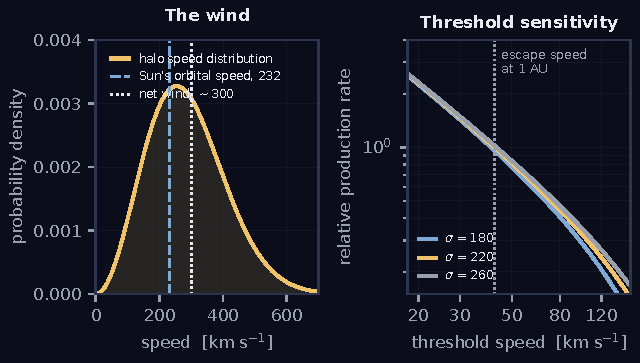
\includegraphics[width=\textwidth]{../figures/fig_wind.pdf}
\caption{The dark matter wind and the threshold sensitivity of the
gravitationally scattered flux. Left: the halo speed distribution with the
Sun's own orbital speed and the resulting net wind speed. Right: the
relative production rate of particles scattered more than 90 degrees, against
the threshold speed, for three assumed velocity dispersions. The rate is
dominated by the slowest particles that can be scattered in at all, which
makes it steeply sensitive to the threshold and only weakly sensitive to the
dispersion.}
\label{fig:wind}
\end{figure}

\section{The dark matter wind}A laboratory on the Earth is stationary with respect
to the Sun, but the Solar System is moving through the galactic halo at
about 220~km\,s$^{-1}$, and the Sun's own motion about the Galactic centre
adds the local Sun's speed of about 232~km\,s$^{-1}$. The result is a
directional flux of dark matter --- the dark matter wind --- with a
characteristic speed of roughly 300~km\,s$^{-1}$\ \idx{Dark matter wind}.

The experimental interest is not the speed, which is well known from
astronomy. It is the direction and the differential. The wind's direction
depends on the Earth's position in its orbit, on the Sun's position in the
galaxy, and on the local halo's velocity distribution. A detector that can
measure the direction of the incoming dark matter can therefore measure
whether the local halo is co-rotating, counter-rotating, or stationary, and
can constrain the velocity distribution in a way no other measurement can.

The obstacle is the obvious one: the Earth's atmosphere, the crust and the
detector itself shield the experiment, and only a small mass of dark matter
gets past. The practical version of the programme uses targets that can be
made thin enough to have a low threshold and that are made of a light
element --- hydrogen, helium, neon -- to maximise the recoil energy. The
threshold, not the flux, is the binding constraint.

\section{Dark matter hail}The same gravitational focusing that produces the capture
also produces a collisionless analogue of rain. Dark matter particles that
are gravitationally scattered by the planets acquire a velocity kick, and
those that are scattered towards the Earth are accelerated into the
atmosphere. The resulting flux is a narrow, directed stream with a
characteristic velocity determined by the escape velocity at the scattering
radius, and its rate depends very steeply on that velocity.

This is where the Solar System's own structure becomes an experimental
handle rather than an obstacle. The cross section for a gravitational
scattering through more than 90 degrees scales as $v^{-4}$, and the halo
speed distribution contributes a factor $v^2$, so the production rate is
dominated by the slowest particles that can be scattered into the Earth at
all. The consequence is a sharp asymmetry: raising the threshold speed from
42 to 120~km\,s$^{-1}$ reduces the rate by a factor of four, whereas
varying the assumed halo velocity dispersion over the whole range from 120 to
400~km\,s$^{-1}$ changes it by about 20 per cent, as
\figref{fig:wind} shows.

That asymmetry is the point of the 2025 proposal. Because the rate is
dominated by a narrow band of speeds just above the threshold, counting the
flux measures the halo's speed distribution in that band with far more
sensitivity than a bulk measurement provides --- and the halo speed
distribution is one of the quantities that also determines how the dark
matter halo responds to the Milky Way's mass \idx{Dark matter hail}.

The difficulty is entirely experimental. The predicted rates are very small,
the required target materials are exotic, and the measurement has to be made
in the presence of a terrestrial flux of ordinary cosmic rays that is
enormously larger.

\section{What this buys the field}Three things, in order of how much they are worth.

The Solar System offers the possibility of a \emph{directional measurement}
that is unique in the field. It offers a \emph{local density measurement}
that tests the halo model in the one place where the density is
significantly enhanced. And it offers a \emph{velocity distribution
measurement} that feeds directly into the interpretation of the laboratory
fluxes, of the halo shape, and of the small-scale structure.

It also offers a caution. The Solar System is a gravitationally complicated
environment, and the dark matter population there is not the ambient halo.
Results obtained with an unbound-stream assumption will not transfer to the
bound population, and the two have different velocities. Chapter~\ref{ch:direct}
returns to this in the context of the neutrino floor, which is in part a
statement about the velocity distribution.

\begin{keytakeaways}
\item Gravitational capture by the Sun and planets enhances the local dark
matter density by four to five orders of magnitude close to the Sun.
\item The dark matter wind is a directed flux with a speed near
300~km\,s$^{-1}$; a directional measurement would constrain the local halo
velocity in a way nothing else can.
\item The dark matter hail proposal turns the steep velocity dependence of
the flux into a measurement of the velocity dispersion.
\item The bound and unbound populations have different velocities, and any
experiment that ignores the distinction will misread its own results.
\end{keytakeaways}
